\documentclass[a4paper,11pt]{article}
% \usepackage{fullpage}
% \usepackage[top=2cm, bottom=2cm, left=2cm, right=2cm]{geometry}
\usepackage[margin=2cm]{geometry}
\usepackage[charter]{mathdesign}
\usepackage{epsfig}
\usepackage{graphicx}
% \usepackage{amssymb}
% \usepackage{amsmath}
\usepackage{verbatim}
\usepackage{fancyhdr}
\usepackage{pifont}% http://ctan.org/pkg/pifont
\usepackage[rgb]{xcolor}
\usepackage{tikz}
\usetikzlibrary{matrix,positioning,fit,shapes,arrows,shadows,calc,backgrounds}
\usepackage{pgfplots}
\usepackage{natbib}
\usepackage{enumitem}
\usepackage{pgfgantt}
\usepackage{booktabs}
\usepackage{url}
\usepackage{xspace}
\usepackage{wrapfig}
\usepackage[show]{chato-notes}
\usepackage{multirow}
\usepackage[official]{eurosym}
\usepackage[bottom]{footmisc}

\usepackage{lipsum}% http://ctan.org/pkg/{graphicx,lipsum}
\newcommand{\PRLsep}{\noindent\makebox[\linewidth]{\resizebox{0.3333\linewidth}{1pt}{$\bullet$}}\bigskip}

\definecolor{verylightmagenta}{rgb}{0.95,0.96,1.0}
\definecolor{brightred}{rgb}{0.90,0.2,0.2}

\newcommand{\ag}[1]{\vspace{1mm}\noindent{\color{orange}{\textbf{Comment:} #1}}}
% \newcommand{\ag}[1]{}
\newcommand{\instructions}[1]{\vspace{1mm}\noindent{\color{blue}{#1}}}
% \newcommand{\instructions}[1]{}

\newcommand{\mpara}[1]{\medskip\noindent{\bf #1}}
\newcommand{\spara}[1]{\smallskip\noindent{\bf #1}}
\newcommand{\acronym}{{\sf\small DIFIAS}\xspace}
\newcommand{\acronymtitle}{{\sf\Large DIFIAS}\xspace}

%\newcommand{\proposaltitle}{{Combating bias and polarization in online media}}
%\newcommand{\proposaltitle}{{Balancing content and reducing controversy in social media}}
\newcommand{\proposaltitle}{{Diversity and fairness in information-access systems}}
\newcommand{\proposalabstitle}{{Diversity and fairness in information-access systems}}

\newcommand{\NP}{{\ensuremath{\mathbf{NP}}}}

% CoG problems
\newcommand{\structure}{{\sc Structure}\xspace}
\newcommand{\dense}{{\sc Dense}\xspace}
\newcommand{\important}{{\sc Important}\xspace}
\newcommand{\event}{{\sc Event}\xspace}
\newcommand{\summarize}{{\sc Summarize}\xspace}

% AdG problems
\newcommand{\model}{{\sc\large Modeling}\xspace}
\newcommand{\discover}{{\sc\large Discovery}\xspace}
\newcommand{\explore}{{\sc\large Exploration}\xspace}
\newcommand{\recommend}{{\sc\large Recommendation}\xspace}
\newcommand{\ui}{{\sc\large UserInterface}\xspace}
\newcommand{\methods}{{\sc\large methods}\xspace}

\newcommand{\rto}{{\bf RT1}\xspace}
\newcommand{\rtw}{{\bf RT2}\xspace}
\newcommand{\rtr}{{\bf RT3}\xspace}

%% squishlist
\newcommand{\squishlist}{\begin{list}{$\bullet$}
  { \setlength{\itemsep}{-1pt}
     \setlength{\parsep}{2pt}
     \setlength{\topsep}{2pt}
     \setlength{\partopsep}{0pt}
     \setlength{\leftmargin}{1.5em}
     \setlength{\labelwidth}{1em}
     \setlength{\labelsep}{0.5em} } }
\newcommand{\squishend}{
\end{list}  }


%% gantt stuff

% \definecolor{foobarblue}{RGB}{0,153,255}
% \definecolor{foobaryellow}{RGB}{234,187,0}
% \newganttchartelement{foobar}{
%     foobar/.style={
%         shape=rounded rectangle,
%         inner sep=0pt,
%         draw=foobarblue!50!black,
%         very thick,
%         top color=white,
%         bottom color=foobarblue!50
%     },
%     foobar incomplete/.style={
%         /pgfgantt/foobar,
%         draw=foobaryellow,
%         bottom color=foobaryellow!50
%     },
%     foobar label font=\slshape,
%     foobar left shift=-.1,
%     foobar right shift=.1
% }

%% tikz stuff

\pgfdeclarelayer{background}
\pgfdeclarelayer{foreground}
\pgfsetlayers{background,main,foreground}


\makeatletter
\tikzset{multicircle/.style  args={#1, #2}{%
 alias=tmp@name, % 
  postaction={%
    insert path={
     \pgfextra{% 
     \pgfpointdiff{\pgfpointanchor{\pgf@node@name}{center}}%
                  {\pgfpointanchor{\pgf@node@name}{east}}%            
     \pgfmathsetmacro\insiderad{\pgf@x}%
     %\foreach \c [count=\ci from = 0, evaluate=\ci as \angle using 360 - (\ci) * #1] in {#2}%
        \fill[white] (\pgf@node@name.center)  circle (\insiderad-\pgflinewidth);%
        \draw[#2] (\pgf@node@name.center)  circle (\insiderad-\pgflinewidth);%
        \fill[#2] (\pgf@node@name.center)  -- ++(0:\insiderad-\pgflinewidth) arc (0:#1:\insiderad-\pgflinewidth)--cycle;%
        }}}}}
\makeatother

\definecolor{yafaxiscolor}{rgb}{0.3, 0.3, 0.3}
\definecolor{yafcolor1}{rgb}{0.4, 0.165, 0.553}
\definecolor{yafcolor2}{rgb}{0.949, 0.482, 0.216}
\definecolor{yafcolor3}{rgb}{0.47, 0.549, 0.306}
\definecolor{yafcolor4}{rgb}{0.925, 0.165, 0.224}
\definecolor{yafcolor5}{rgb}{0.141, 0.345, 0.643}
\definecolor{yafcolor6}{rgb}{0.965, 0.933, 0.267}
\definecolor{yafcolor7}{rgb}{0.627, 0.118, 0.165}
\definecolor{yafcolor8}{rgb}{0.878, 0.475, 0.686}
\definecolor{yafcolor9}{rgb}{0.965, 0.733, 0.767}

\newlength{\yafaxispad}
\setlength{\yafaxispad}{-4pt}
\newlength{\yaftlpad}
\setlength{\yaftlpad}{\yafaxispad}
\addtolength{\yaftlpad}{-0pt}
\newlength{\yaflabelpad}
\setlength{\yaflabelpad}{-2pt}
\newlength{\yafaxiswidth}
\setlength{\yafaxiswidth}{1.2pt}
\newlength{\yafticklen}
\setlength{\yafticklen}{2pt}

\makeatletter
\def\pgfplots@drawtickgridlines@INSTALLCLIP@onorientedsurf#1{}
\makeatother

\newcommand{\yafdrawxaxis}[2]{
	\pgfplotstransformcoordinatex{#1}\let\xmincoord=\pgfmathresult 
	\pgfplotstransformcoordinatex{#2}\let\xmaxcoord=\pgfmathresult 
	\pgfsetlinewidth{\yafaxiswidth} 
	\pgfsetcolor{yafaxiscolor}
	\pgfpathmoveto{\pgfpointadd{\pgfpointadd{\pgfplotspointrelaxisxy{0}{0}}{\pgfqpointxy{\xmincoord}{0}}}{\pgfqpoint{-0.5\yafaxiswidth}{\yafaxispad}}}
	\pgfpathlineto{\pgfpointadd{\pgfpointadd{\pgfplotspointrelaxisxy{0}{0}}{\pgfqpointxy{\xmaxcoord}{0}}}{\pgfqpoint{0.5\yafaxiswidth}{\yafaxispad}}}
	\pgfusepath{stroke}

}
\newcommand{\yafdrawyaxis}[2]{
	\pgfplotstransformcoordinatey{#1}\let\ymincoord=\pgfmathresult 
	\pgfplotstransformcoordinatey{#2}\let\ymaxcoord=\pgfmathresult 
	\pgfsetlinewidth{\yafaxiswidth} 
	\pgfsetcolor{yafaxiscolor}
	\pgfpathmoveto{\pgfpointadd{\pgfpointadd{\pgfplotspointrelaxisxy{0}{0}}{\pgfqpointxy{0}{\ymincoord}}}{\pgfqpoint{\yafaxispad}{-0.5\yafaxiswidth}}}
	\pgfpathlineto{\pgfpointadd{\pgfpointadd{\pgfplotspointrelaxisxy{0}{0}}{\pgfqpointxy{0}{\ymaxcoord}}}{\pgfqpoint{\yafaxispad}{0.5\yafaxiswidth}}}
	\pgfusepath{stroke}
}

\newcommand{\yafdrawaxis}[4]{\yafdrawxaxis{#1}{#2}\yafdrawyaxis{#3}{#4}}

\pgfplotscreateplotcyclelist{yaf}{% 
{yafcolor1,mark options={scale=0.75},mark=o}, 
{yafcolor2,mark options={scale=0.75},mark=square},
{yafcolor3,mark options={scale=0.75},mark=triangle},
{yafcolor4,mark options={scale=0.75},mark=o},
{yafcolor5,mark options={scale=0.75},mark=o},
{yafcolor6,mark options={scale=0.75},mark=o},
{yafcolor7,mark options={scale=0.75},mark=o},
{yafcolor8,mark options={scale=0.75},mark=o}} 

\pgfplotsset{axis y line=left, axis x line=bottom,
	tick align=outside,
	compat = 1.3,
	tickwidth=\yafticklen,
	clip = false,
	every axis title shift = 0pt,
    x axis line style= {-, line width = 0pt, opacity = 0},
    y axis line style= {-, line width = 0pt, opacity = 0},
    x tick style= {line width = \yafaxiswidth, color=yafaxiscolor, yshift = \yafaxispad},
    y tick style= {line width = \yafaxiswidth, color=yafaxiscolor, xshift = \yafaxispad},
    x tick label style = {font=\scriptsize, yshift = \yaftlpad},
    y tick label style = {font=\scriptsize, xshift = \yaftlpad},
    every axis y label/.style = {at = {(ticklabel cs:0.5)}, rotate=90, anchor=center, font=\scriptsize, yshift = -\yaflabelpad},
    every axis x label/.style = {at = {(ticklabel cs:0.5)}, anchor=center, font=\scriptsize, yshift = \yaflabelpad},
    x tick label style = {font=\scriptsize, yshift = 1pt},
    grid = major,
    major grid style  = {dash pattern = on 1pt off 3 pt},
	every axis plot post/.append style= {line width=\yafaxiswidth} ,
	legend cell align = left,
	legend style = {inner sep = 1pt, cells = {font=\scriptsize}},
	legend image code/.code={%
		\draw[mark repeat=2,mark phase=2,#1] 
		plot coordinates { (0cm,0cm) (0.15cm,0cm) (0.3cm,0cm) };% 
	} 
}



\pagestyle{fancy}
\lhead[{Gionis}]{{Gionis}}
\rhead[{\acronym}]{{\acronym}}
\chead[~]{{~}}
% \setcounter{page}{1}

\renewcommand{\baselinestretch}{1.01} 
\begin{document}


\begin{center} 
{\large Vetenskapsrådet: Distinguished professor grant within natural % } \vspace{1mm}\\ 
% {\large 
and engineering sciences 2024} \vspace{2.5mm}\\
{\Large Research plan} \vspace{2mm}\\
{\LARGE\bf {\proposaltitle} {\sc (}{\acronymtitle}{\sc )}}  \vspace{3mm} \\
{\Large Aristides Gionis}  \\
\end{center}

\subsection*{1.~~~Purpose and aims}

In the modern information age we are submersed in a constant stream of data from various sources, 
ranging from the internet and social media to news outlets and podcasts. 
While this wealth of information has the potential to empower individuals, 
it also poses a significant challenge known as \emph{information~overload}:
as the volume of available information continues to grow exponentially, 
individuals are increasingly struggling to sift through noisy data
to find reliable, relevant, and meaningful~content.

\iffalse
This overload can lead to decision paralysis, reduced productivity, and cognitive overload, ultimately hindering our ability to make informed decisions and engage critically with the world around us. Addressing the problem of information overload requires not only technological solutions such as improved search algorithms and filtering mechanisms but also a concerted effort to cultivate digital literacy skills and promote mindful consumption habits among individuals.
\fi 

To mitigate the problem of information overload, 
in addition to cultivating % digital literacy skills and promoting 
mindful consumption habits, 
it also requires \emph{technological solutions} tailored to the needs of individuals. 
Advanced information-retrieval algorithms can help streamline search processes, 
enabling users to find relevant content. 
%  more efficiently amidst vast data pools. 
Recommendation systems play a crucial role by suggesting personalized content 
based on users' preferences and past interactions. 
The challenge of information overload arises in various scenarios. 
For instance, it occurs when users interact with search engines using keyword searches, 
when peruse product reviews, 
scroll through social-media timelines, or 
receive recommendations for movies or restaurants.

%  thus reducing the burden of sifting through irrelevant information. 
% Personalization further enhances user experiences by tailoring content delivery to individual interests and behaviors, ensuring that users receive the most pertinent information. 
% By harnessing these technological tools, we can navigate the information landscape more effectively, mitigating the challenges posed by information overload and empowering individuals to make informed decisions.

When designing smart tools for infromation access, ensuring \emph{relevance} is paramount:
users expect content that aligns closely with their interests and needs.
But beyond relevance, \emph{diversity} and \emph{fairness} are equally crucial.
Diversity ensures exposure to varied perspectives, 
while fairness ensures equitable access to information.
Integrating diversity and fairness into information-access systems has numerous benefits, 
such as mitigating biases, 
helping counter filter-bubble and rabbit-hole effects, 
fostering a more inclusive and fair representation of different perspectives, and 
promoting a well-rounded understanding of topics.

While relevance, diversity, and fairness
have been extensively studied in different areas of computer science, 
including information retrieval, recommender systems, and machine learning,
their interplay remains relatively understudied.
We posit that incorporating diversity and fairness into modern information-access systems
remains an unsolved problem, 
offering ample space for fundamental research contributions.
The \acronym\ project aspires to contribute in addressing 
significant challenges in this area. 
% More concretely, the project has the following goal.

\medskip
\noindent
\hspace{-3mm}\colorbox{verylightmagenta}{
\begin{minipage}{\textwidth}
{\bf High-level goal of \acronym:} 
We will develop theoretical foundations and novel abstractions to 
study notions of diversity and fairness in information-access systems.
We will design algorithms for these problems with provable guarantees.
Among diffrent information-access systems we will focus on 
information-exploration systems, information networks, and two-sided information markets.
\end{minipage}}

\ag{Text below could also go to ``novelty''.}

\spara{Challenges.}
The proposed project is of theoretical nature, 
lying in the areas of information retrieval, recommender systems,  
knowledge discovery, and algorithms design. 
Achieving the project aim entails significant challenges. 
First, we need to design novel abstractions that model faithfully system entities and their interactions, 
e.g., semantic distances between content items or user behavior, 
while capturing notions of diversity and fairness and their inter-play with relevance.
Second, we will be dealing with noisy data generated by a diverse set of actors
who exhibit complex behavior and may have adversarial motives, 
thus, our methods need to be robust to such complexities.
Third, we will be confronted with challenging optimization tasks, and thus, 
we will need to develop scalable algorithms with theoretical guarantees on the solution quality.

\iffalse
\medskip
\noindent
\hspace{-3mm}\colorbox{verylightmagenta}{
\begin{minipage}{\textwidth}
{\bf Hypothesis:} 
We postulate that modern information-access systems suffer from lack of diversity 
and unfair representation of content. 
We hypothesize that such deficiencies can be mitigated by formulating novel abstractions
and designing rigorous computational methods to support individuals in 
maximizing diversity and improving fairness of the available content. 
\end{minipage}}
\fi

\spara{Objectives.}
Our overarching objective is to address deficiencies of modern information-access systems 
with regard to lack of diversity and unfair representation of content.
To achieve this objective we aim to consolidate existing approaches, 
including our recent and ongoing work,  
and push the state-of-the-art 
in terms of introducing novel abstractions, 
developing rigorous computational methods, and 
performing evaluations on real-world applications.
In particular, {\acronym} has the following research objectives. 
%
\begin{description}
\setlength{\itemsep}{-4pt}
\item[{Models and problems:}]
Develop novel models and novel problem formulations that enable 
obtaining a deeper understanding on phenomena related 
to lack of diversity and fairness in  modern information-access systems.
Focus on three specific domains: 
\emph{information-exploration systems}, \emph{information networks}, and 
\emph{two-sided information markets}.

\item[{Algorithms:}]
Develop computational methods for the formulated problems.
Our methods will be designed for different computational settings, 
e.g., combinatorial formulations, stochastic and uncertain data, 
reinforcement learning, algorithms with predictions, and more.
The proposed algorithms should be efficient %, 
% should be able to deal with uncertainty, 
and should offer theoretical guarantees.

% \item[\manet\ {Limitations:}] Study the proposed structure-discovery problems under the different computational models in order to understand their fundamental limitations, and  develop hardness results or lower bounds.

\item[{Applications:}]
Apply the developed methodology on different application scenarios 
and evaluate the resulting algorithms on real-world benchmark datasets.
% Validate proof-of-concept by showcasing findings of the methods on different use cases. 
Implement the developed algorithms and make them available to the scientific community.

\item[{Research environment in KTH:}]
Strengthen the area of algorithmic data analysis 
at the department of computer science in KTH. 
Nurture doctoral students and postdoctoral researchers in the topic of the project,
and create synergies with other faculty working on 
the foundations of data science, machine learning, and artificial intelligence.
\end{description}

\spara{Diversity vs.\ fairness.}
Diversity maximization and fairness assurance are both important considerations in machine learning.
While they share some common goals, such as promoting inclusivity and reducing discrimination, 
they address different dimensions and require distinct methodologies and techniques. 

Diversity maximization often relies on optimizing distance-based or coverage-based objectives, 
designed to ensure that the outputs generated by a system cover a wide range of perspectives
and promote heterogeneity. 
Diversity maximization is often applied in recommendation systems, search engines, 
and other decision-making systems where providing a diverse set of options or perspectives is desirable.

On the other hand, 
fairness aims to mitigate biases and ensure equitable treatment of individuals or groups.
Fairness methods are based on ensuring or optimizing fairness criteria, or post-processing techniques. 
Fairness is often studied in contexts where decisions may impact individuals or groups differently, 
and finds applications in domains such as hiring, criminal justice, and healthcare.

In this project we consider that fairness concepts can be extended to other contexts,  
beyond individuals and demographic groups. 
For instance, we can talk about fairness in the context of news recommender systems, 
asking to ensure that a set of recommender news articles represent fairly the political spectrum.
In this way, similar to diversity, we can study fairness in the context of different information-access systems. 
Note however that diversity alone does not guarantee fairness, 
and fairness considerations may extend beyond simply ensuring diversity 
in the outputs of a machine learning model.

\subsection*{2.~~~State of the art}

Maximizing diversity and promoting fairness have been studied 
extensively in different contexts in computer science, 
especially in recent times with the raising importance of \emph{responsible AI}~\cite{dignum2019responsible}.
Due to space limitations we only discuss some representative approaches, 
and their connection with this proposal.

% \spara{diversity as an optimization problem}

From the theoretical viewpoint, the literature mainly focuses on two notions of diversity: 
\emph{coverage-based diversity}, relying on \emph{submodular} coverage functions~\cite{bach2013learning} 
and \emph{pairwise dissimilarity-based} diversity, like \emph{dispersion}~\cite{hassin1997approximation}.
Researchers have also attempted to formulate \emph{axioms} of diversity and study
their implications~\cite{gollapudi2009axiomatic}. 
A particularly appealing formulation is the \emph{max-sum diversity} problem~\cite{borodin2012max},
which captures trade-off between diversity and relevance for item-selection problems.
Solutions for max-sum diversity involve \emph{combinatorial methods}~\cite{borodin2012max},
\emph{convex programming}~\cite{cevallos2016max} and 
\emph{local search}~\cite{cevallos2019improved}, among other.
Such formulations and techniques will be a basis for {\acronym}
to study extensions and improved methods. 

% \spara{diversity in recommender systems}

Diversity has also been acknowledged as a crucial component in \emph{recommender systems},
shown to improve user experience~\cite{Castells2022}, 
and thus, it has received considerable attention recently. 
% ~\cite{on_unexpectedness, improving_aggregate, evaluating_novel_recs, diversity_top_n_recs, rank_relevance}.
One of the most popular methods in \emph{information retrieval},
seeking to strike a balance between diversity and relevance, 
is the \emph{maximal marginal relevance} (MMR)~\cite{MMR}, 
while many other strategies have proposed to 
maximize some utility function that combines relevance and diversity~\cite{DUM,DPMF}.
% based on submodular functions~\cite{DUM}, probabilistic matrix factorization~\cite{DPMF},  and other.
In \acronym we aim to extend the state-of-the-art significantly, 
by incorporating models of \emph{user behavior}, 
investigating approaches based \emph{reinforcement learning}, 
and studying novel notions for \emph{fair representation} of recommended items. 

% \spara{diversity in graphs}

Diversity and fairness in graph settings is a significantly less studied area,
compared to item-selection and recommender-systems problems.
Still several ideas have been investigated, 
such as \emph{adding} or \emph{rewiring graph edges} for
\emph{reducing polarization}~\cite{adriaens2023minimizing,cinus2023rebalancing,haddadan2022reducing},
\emph{mitigating exposure to harmful content}~\cite{coupette2023reducing,fabbri2022rewiring}, 
or \emph{improving fairness for the Page\-Rank algorithm}~\cite{tsioutsiouliklis2022link}.
Extending this line of work for diversity and fairness in graphs
by introducing new models and methods
is a central goal of the \acronym project.
Finally, while there is a growing literature for content recommender systems, 
algorithmic recommendations in social media~\cite{wang2021user}, 
the study of diversity and fairness in this context is largely unexplored topic.

% \spara{fairness in ML}

The topic of bias and fairness in machine learning has received a lot of interest in the recent years, 
having spawn a large community and dedicated dissemination venues, such as the FAccT Conference. 
While many surveys and tutorials can be found online~\cite{caton2020fairness,mehrabi2021survey}, 
we note that our project is more closely related to notions of
\emph{bias and fairness in unsupervised machine learning}, 
such as 
\emph{fair clustering}~\cite{chierichetti2017fair}, 
\emph{diversity-aware clustering}~\cite{thejaswi2021diversity}, 
and \emph{fair graph mining}~\cite{dong2023fairness}.

% \spara{my work}

Notably, together with my team and research collaborators, 
we have pioneered work on many of the above topics,
including
different formulations for diversity in network analysis~\cite{adriaens2023minimizing,cinus2023rebalancing,coupette2023reducing,oettershagen2024finding}
diversity in ranking problems~\cite{zhang2022ranking}, 
as well as in data clustering~\cite{thejaswi2021diversity}.

\subsection*{3.~~~Significance and scientific novelty}

\instructions{
Describe briefly how the project relates to previous research within the area, 
and the impact the project may have in the short and long term. 
Describe also how the project moves forward or innovates the current research frontier.}

\ag{
Maybe some comments from state of the art can be moved here, or rephrased. \\
Also say the main novelty would be to study diversity and fairness in new settings.
}

\subsection*{4.~~~Project description}


\subsubsection*{4.1.~~~Theory and methods}

The project is structured along three {\em research themes}:
\vspace{-1mm}
\begin{description}
\setlength{\itemsep}{-4pt}
\item[{\exploration}\,:] 
diversity and fairness for information exploration tasks;
\item[{\networks}\,:]
diversity and fairness in information networks; and 
\item[{\markets}\,:]
diversity and fairness in information markets.
\end{description}
\vspace{-1mm}
\iffalse
\emph{diversity and fairness for information exploration tasks} (\exploration), 
\emph{diversity and fairness in information networks} (\networks), 
\emph{diversity and fairness in information markets} (\markets), 
\fi
Each theme is characterized by a different domain
for which we are aiming to ensure criteria of diversity and fairness. 
Each domain corresponds to a distinct family of information-access systems, 
has its own unique characteristics, 
it will be modeled using different abstractions, 
and we will employ different methods and techniques for solving the corresponding 
computational tasks. 
On the other hand, connections do exist, 
for instance, common definitions for diversity and fairness will be used, 
and thus, we will seek to identify synergies between the three themes
and adopt ideas that turn out to be successful.

With respect to methods, 
emphasis will be given to combinatorial algorithms,
building on the previous work of the PI 
on developing combinatorial methods for data-analysis problems.
In particular, we will consider techniques such as 
combinatorial optimization, 
optimization of submodular functions, 
local-search methods, 
greedy algorithms, 
dynamic pro\-gram\-ming, 
linear-pro\-gram\-ming and semi\-def\-ini\-te-pro\-gram\-ming relaxations, 
primal-dual methods, convex optimization,
stochastic gradient descent, etc. 
Furthermore, we will explore ideas in new domains, 
such as 
algorithms with predictions~\cite{mitzenmacher2022algorithms} and
reinforcement learning.

Next we overview the three research themes of \acronym.


\subsubsection*{Research theme 1: Diversity and fairness for information-exploration tasks}

\noindent
\hspace{-3mm}\colorbox{verylightmagenta}{
\begin{minipage}{\textwidth}
\ag{do we need a summary in a box?}
\end{minipage}}

\vspace{2mm}
We consider an information system
that stores a large collection of information items.
Users interact with the system and can access the items through various means 
such as keyword searches, recommendations, or combinations of those.
We assume that users have different interests
and the system has prior information about user interests and user behavior.
Note that this is a general setting that can be used to model different scenarios, 
for instance, web-search engines, e-commerce systems, video-sharing platforms, 
or platforms for browsing and reading news articles.
Our objective is to design methods that enable users to 
\emph{explore the available information items in the system} through their interaction.
We are interested in systems that offer items that are relevant to the user's interests, 
but also satisfy criteria of diversity and fairness of representation.

As discussed before, combining relevance with diversity is an archetypal problem
in information retrieval and recommender systems, 
and there is a plethora of methods to address it. 
However, the majority of methods assume very simplistic models;
for instance, \emph{find a set of $k$ items} 
that optimize some function that combines relevance with diversity. 
In the real world, information-exploration tasks are significantly more complex and more nuanced. 
First, items are presented to users in an order, and not as a set.
Second, users may click on some of the presented item, 
initiating a new ``round'' of exploration. 
Third, there is chance that users terminate their interaction with the system, 
based on the relevance and novelty of the presented items,
as well as the duration of the exploration session so far.

Motivated by these observations, 
we will formulate novel frameworks for information exploration
that model \emph{user behavior} and aim to optimize 
the total amount of knowledge accrued by the user during exploration, 
while accounting for relevance and diversity.
In our preliminary work, we have studied a simple version 
of this problem where we ask to \emph{maximize expected diversity} 
in presence of a probability that, depending on item relevance,  
at any given step the user will terminate the exploration task. 
The problem has very interesting connections to \emph{ordered Hamiltonian-path problem}, 
and under mild assumptions we are able to design provable approximation algorithms.


Tianyi 








This thrust builds strongly on our preliminary work.
In particular, we have considered the problem 
of identifying controversial discussions on social media~\cite{garimella2018quantifying}.
Our methods are designed to be applicable to topics in any domain 
(e.g., political, economical, or cultural), and in a general setting.
We have also addressed the question of devising a measure of controversy,
which is applicable to any online discussion.
More recently we devised a new study aimed to 
understand the phenomenon of echo chambers in social media, 
and to characterize distinct user types and their role in their local community~\cite{garimella2018political}.

\smallskip
In this project we will extend significantly our problem representations
so as to obtain a deeper analysis and develop much more advanced knowledge-discovery methods.
In particular, our existing work relies on analyzing plain graphs
with no additional information regarding text or time. 
In \acronym\ we will incorporate text information into the mining process.
We will develop methods to extract semantic annotations from the textual data, 
such as
($i$) agreement between users; 
($ii$) political leaning of users or content items; 
($iii$) stance with respect to topics; 
and so on.
We will use this information to enrich our graph models,
provide novel formulations for mining semantically-annotated graphs, 
and then design efficient algorithms.

\smallskip
As an example, we will consider discussion graphs
where edges are annotated with agreement (`$+$') or disagreement (`$-$'), 
and thus, represented as {\em signed graphs}.
In this setting we will consider the problems of discovering alliances 
(dense subgraphs with many `$+$' and few `$-$' edges) 
or conflicting communities
(sets of vertices with many `$+$' and few `$-$' within sets and many `$-$' and few `$+$' across sets). 
These are novel problems related to dense-subgraph discovery~\cite{rozenshtein2014event,sozio2010community-search,tatti2015density,tsourakakis2013denser}
and correlation clustering~\cite{bansal2004correlation,gionis2007clustering}.

\smallskip
We will also leverage the temporal dimension of the data
and study formulations that allow to model and discover 
bias, polarization, and conflict in the setting of temporal networks.
This thread will make strong connections with our previous work on 
temporal networks~\cite{rozenshtein2016temporal, rozenshtein2016reconstructing, rozenshtein2017finding}
Finally we will consider problem representations  
related to motif discovery~\cite{aslay2018mining,coletto2017motif} and role mining~\cite{arockiasamy2016combinatorial} 
in the context of \acronym.





\subsubsection*{4.2.~~~Time plan and implementation}

\instructions{
Describe summarily the time plan for the project during the grant period, 
and how the project will be implemented. 
Describe also any crucial risks or obstacles that may impact on the implementation, 
and your plan for managing these.}


\subsubsection*{4.3.~~~Project organisation}

\instructions{
Clarify the contributions of yourself and any other researchers and/or key persons (including any doctoral students) 
to the implementation of the project, 
including a description of competences and roles in the project. 
Explain in particular how the time allocated by you (that is, your activity level) 
as project leader is suitable for the task, 
including the relationship with your other research undertakings.}

\subsection*{5.~~~Need for research infrastructure}

\instructions{
Specify the project’s need for international and national research infrastructure. 
If you choose to use other infrastructures than those supported by the Swedish Research Council, 
and that are thereby open to all, 
you must justify this (also applies to local research infrastructure).}

\subsection*{6.~~~International and national collaboration}

\instructions{
Describe your collaboration with foreign and Swedish researchers and research teams. 
State whether you contribute to or refer to international collaboration in your research.}


%%%%%%%%%%%%%%%%%%%%%%%%%%%%%%%%%%%%%%%%%%%%%%%%%%%%%%%%%%%%%%%%%%
%%%%%%%%%%%%%%%%%%%%%%%%%%%%%%%%%%%%%%%%%%%%%%%%%%%%%%%%%%%%%%%%%%
%%%%%%%%%%%%%%%%%%%%%%%%%%%%%%%%%%%%%%%%%%%%%%%%%%%%%%%%%%%%%%%%%%
%%%%%%%%%%%%%%%%%%%%%%%               %%%%%%%%%%%%%%%%%%%%%%%%%%%%
%%%%%%%%%%%%%%%%%%%%%%%    REBOUND    %%%%%%%%%%%%%%%%%%%%%%%%%%%%
%%%%%%%%%%%%%%%%%%%%%%%               %%%%%%%%%%%%%%%%%%%%%%%%%%%%
%%%%%%%%%%%%%%%%%%%%%%%%%%%%%%%%%%%%%%%%%%%%%%%%%%%%%%%%%%%%%%%%%%
%%%%%%%%%%%%%%%%%%%%%%%%%%%%%%%%%%%%%%%%%%%%%%%%%%%%%%%%%%%%%%%%%%
%%%%%%%%%%%%%%%%%%%%%%%%%%%%%%%%%%%%%%%%%%%%%%%%%%%%%%%%%%%%%%%%%%

\newpage
\begin{center}

{\LARGE\bf REBOUND} % \vspace{2mm}\\ 
\end{center}


\subsection*{Section a. Background and objectives}

Social media play a critical role in today's information society, 
not only by connecting people with their friends, 
but also by providing a medium where information is disseminated and public opinion is shaped.
Initially it seemed that giving ordinary citizens the means to create content of their own
and share their opinion publicly 
can have only positive effects: increase the exposure to diverse ideas
and improve the democratic process.
However, during the past few years we have witnessed that
the rise of online media has led to 
a series of undesirable phenomena, 
such as creation of information silos and increased polarization.
More and more digital citizens find themselves in online environments
where they only see opinions that confirm their preexisting beliefs,
and as a result, they become ideologically segregated.

\smallskip
These negative aspects of social media have drawn a lot of attention recently.
There has been a considerable amount of criticism, skepticism, 
discussion in public forums, as well as calls % from stakeholders 
to fix the problems. 
Prominent media outlets, researchers, and think tanks have contemplated whether 
``{\em social media is a threat to democracy}.''%
\footnote{For example, see www.economist.com/leaders/2017/11/04/do-social-media-threaten-democracy,\\
or www.weforum.org/agenda/2016/08/the-biggest-threat-to-democracy-your-social-media-feed/}
Given all these concerns a natural question arises.

\smallskip
{\em How can we address the deficiencies encountered in today's online platforms  
and how can we create environments in which online media 
enable exchange of alternative views and promote constructive deliberation?}

\smallskip
This is certainly a complex problem that requires
parallel work and cooperation of multiple parties: 
owners of social-media platforms and
traditional media outlets, 
journalists,
policy makers, 
educators, 
as well as independent academics. 
It is also a cross-disciplinary research challenge that requires expertise in 
sociology, political science, economics, engineering, design, and {\em computer science}.

\smallskip
The \acronym\ project aspires to contribute in addressing this complex problem
by designing methods to perform large-scale data analysis so as to shed light to 
phenomena such as bias, polarization, conflict, and 
information silos in online media. 
It will also contribute with methods
that give users easier access to opposing ideas
and incentives to explore and understand alternative view\-points. 
More concretely, the project has the following goal.

\medskip
\noindent
\hspace{-3mm}\colorbox{verylightmagenta}{
\begin{minipage}{\textwidth}
{\bf High-level goal of \acronym:} 
We will develop theoretical foundations and a concrete set of algorithmic techniques 
to address deficiencies in today's online media.
We will develop methods to discover structure and patterns 
of segregation, conflict, and closeness in social-media systems.
We will address the issues of 
reducing bias and po\-lar\-iza\-tion, breaking information silos,
and creating awareness of users to explore alternative view\-points.
\end{minipage}}

\spara{Challenges.}
Achieving the project goal is an extremely challenging task for a number of reasons. 
First, we will be dealing with noisy data, 
generated by a diverse set of actors
who exhibit complex behavior and may have adversarial motives.
Additionally, data are highly dynamic:
new events are taking place and inter\-actions between actors 
are constantly evolving over time. 
Second, we will deal with concepts that are not well-understood 
and we will need to develop novel abstractions. %  and problem definitions. 
% As a simple example, although one may have an
% intuitive understanding of the claim ``{\em social media amplify the problem of echo chambers},''
% there is no well-accepted definition for what constitutes an echo chamber, 
% nor how to measure it.
For instance, 
while there is a well-motivated discussion 
about how to combat the problem of bias and polarization in online media, 
there is no understanding of what does this entail % , what are the trade-offs, 
nor what could be the side effects of possible remedial actions.
Third, we will be confronted with challenging computational tasks 
that lead to difficult optimization problems. 
Thus, it is desirable to develop methods 
that offer approximation guarantees or other theoretical properties. 

\iffalse
\spara{Methodological approach.}
We will pursue the project goal by
following a methodology that aims to tackle the challenges outlined above.
(1)~We will develop abstractions that capture the semantics of the application domain
and we will provide formal problem definitions that capture our objectives.
(2)~We will develop and work with theoretical frameworks that capture the noise and complexity 
of real-world data. 
(3)~We will develop scalable algorithms with theoretical guarantees on the solution quality. 
\fi

\spara{Hypothesis and objectives.}
%
% Our encompassing research objective is to 
% develop a rigorous methodology in order to address 
% deficiencies in today's online media, such as 
% bias, conflict, and information silos. 
The project is grounded on the following hypothesis. 

\medskip
\noindent
\hspace{-3mm}\colorbox{verylightmagenta}{
\begin{minipage}{\textwidth}
{\bf Hypothesis:} 
We postulate that bias, conflict, polarization, and information silos
are real phenomena in today's online media. 
We hypothesize that these deficiencies can be alleviated by designing and building appropriate tools, 
and that people can get interested to explore and engage with alternative viewpoints. 
\end{minipage}}

\medskip
Our encompassing research objective is to test this hypothesis.
To achieve this objective we aim to consolidate existing approaches, 
including our recent work, 
and push significantly the state-of-the-art 
in terms of models, novel problem formulations, 
improved algorithmic techniques, and applications.
In particular, {\acronym} has the following concrete objectives. 
%
\begin{description}
\setlength{\itemsep}{-1pt}
\item[{Models:}]
Develop novel models for analyzing data on news dissemination and online discussions in online media, 
with the aim to obtain a deeper understanding on phenomena related to bias, polarization, and 
information bottlenecks.
Extend standard data-mining problem formulations for this particular application domain, 
and formulate novel problem representations for the tasks specified in the three research thrusts of the project.

\item[{Algorithms:}]
Develop efficient algorithmic solutions for the formulated problems.
Our algorithms should take into account the rich available data representations
as well as the stochastic and noisy nature of the problem domain.
The proposed algorithms should be efficient, 
should be able to deal with uncertainty, and should offer theoretical guarantees.

% \item[\manet\ {Limitations:}] Study the proposed structure-discovery problems under the different computational models in order to understand their fundamental limitations, and  develop hardness results or lower bounds.

\item[{Applications:}]
Apply the developed methodology on different application scenarios 
and evaluate the resulting algorithms on real-world datasets.
Validate proof-of-concept by showcasing findings of the methods on different use cases. 
Implement the developed algorithms and make them available to the scientific community.

\item[{Education:}]
Nurture doctoral students and postdoctoral researchers.
Educate them about fundamental algorithmic techniques,
teach them the value of identifying important data-analysis problems, 
and support them becoming independent researchers.
\end{description}

% \todo{access to data}

\spara{State of the art.}
%
%% Bias and polarization in general, mechanisms
%
% The study of the phenomena of bias and polarization 
% predates the era of the internet and social media.
% The first works appear in the fields of psychology, 
% social science, and political science. 
A number of theories have been proposed in psychology and social sciences 
in an attempt to {\em explain the mech\-a\-nisms} that result in various types
of bias that are present in our society. 
Those include the theories of 
{\em cognitive dissonance}~\cite{festinger1962theory}, 
\emph{selective exposure}~\cite{frey1986recent}, and
\emph{biased assimilation}~\cite{lord1979biased}. 
All these psychological mech\-a\-nisms, 
together with other biases, such as, 
\emph{algorithmic filtering} and \emph{personalization}~\cite{bozdag2013bias}, 
are connected to the phenomenon of information silos and echo chambers
in online media~\cite{pariser2011filter}.
% Understanding how all these phenomena interact with each other and the precise
% causality relations is an open research domain.
% 
% \smallskip
With the wide availability of online media data, 
a lot of work has been devoted in studying 
controversy, polarization, bias, and conflict in social media. 
In one of the first papers, Adamic and Glance
study the link structure of blog posts on the 2004 US presidential election;
they provide evidence that conservative blogs are linking 
to each other more frequently and in a denser pattern~\cite{adamic2005political}. 
Conover et al.\ study twitter data from congressional midterm elections
and identify a highly-segregated partisan network structure
by the means of graph partitioning~\cite{conover2011political}. 
% Guerra et al.\ propose an alternative graph-structure measure 
% based on the analysis of the boundary between communities~\cite{guerra2013measure}, 
% while Morales et al.\ apply graph-diffusion techniques~\cite{morales2015measuring}. 

\smallskip
Echo chambers have been shown to exist in various forms of online media such as 
blogs~\cite{gilbert2009blogs,wallsten2005political}, forums~\cite{edwards2013participants}, and 
social-media sites~\cite{barbera2015tweeting,gromping2014echo,quattrociocchi2016echo}.
An et al.\ analyzed the activity of twitter users who engage with political news
and found that 90\% of the users directly follow news media of only one political leaning~\cite{an2014sharing}. 
In a study performed in Facebook, Bakshy et al.\
% measure the degree to which users with declared political affiliations 
% consume cross-cutting content, i.e., 
% content predominantly posted by users of opposing political affiliation~\cite{bakshy2015exposure}.
% They 
find that although users are exposed to a significant amount of cross-cutting content, 
they opt to engage with proportionately less cross-cutting content~\cite{bakshy2015exposure}.
% 
% \smallskip
A few recent papers have addressed the problem of 
mitigating polarization and diffusing echo chambers. 
The underlying ideas involve making users aware 
of other users' stance on a given issue~\cite{liao2014can,liao2014expert}, 
or revealing the bias of the news articles they read~\cite{munson2013encouraging}.
In work pioneered in my research group, 
we have studied the problem of reducing bias and polarization
by the means of 
recommending links of users to follow~\cite{garimella2017reducing},
selecting users to promote campaigns~\cite{garimella2017balancing},
and maximizing diversity~\cite{diversity-cascade,diversity-static}.

\smallskip
In summary, the problem of reducing bias and polarization in online information
has already received some attention in the literature.
However, the area is still largely undeveloped and most works are preliminary.
The topic has attracted a lot of attention in the public discussion forum, 
and there is exciting work ahead to be done in a range of disciplines, 
including with no doubt computer science.


\subsection*{Section b. Methodology}

\begin{figure}[t]
\begin{center}
{\scalebox{0.96}{\small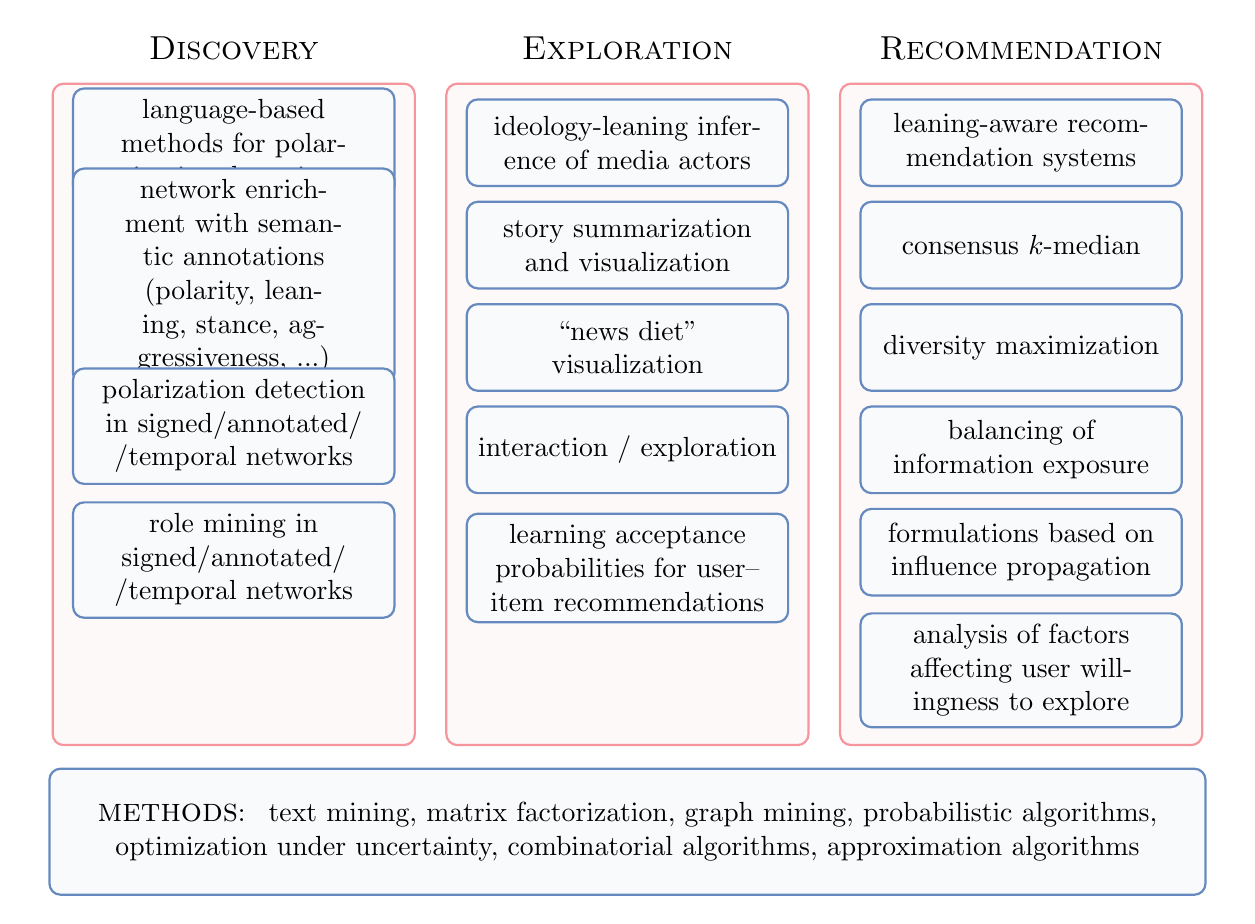
\begin{tikzpicture}
  [auto,
  frame/.style ={draw=yafcolor4!50, fill=yafcolor4!03, thick, inner sep=0em, rounded corners, text centered,
    text width=4.6cm, minimum height=8.4cm},
  block/.style ={draw=yafcolor5!70, fill=yafcolor5!03, thick, inner sep=0.4em, rounded corners, text centered,
    text width=3.8cm, minimum height=1.1cm}, 
  plaintext/.style = {text width=1.8cm, text centered},
  widetext/.style = {text width=5cm, text centered},    
  ]

\tikzstyle{simpleline} = [color=yafcolor4!70, thick, dashed]

\node[frame] (f1) at (5,2.55) {};
\node[widetext] (rh1) at (5,7.2) {\discover};

\node[block] (b11) at (5,6)   { language-based methods for polarization detection } ;
\node[block] (b12) at (5,4.3) { network enrichment with semantic annotations\\(polarity, leaning, stance, aggressiveness, ...) } ;
\node[block] (b13) at (5,2.4) { polarization detection in signed/annotated/ /temporal networks } ;
\node[block] (b14) at (5,0.7) { role mining in signed/annotated/ /temporal networks } ;


\node[frame] (f2) at (10,2.55) {};
\node[widetext] (rh2) at (10,7.2) {\explore};

\node[block] (b21) at (10,6)   { ideology-leaning inference of media actors } ;
\node[block] (b21) at (10,4.7) { story summarization and visualization } ;
\node[block] (b23) at (10,3.4) { ``news diet'' visualization } ;
\node[block] (b24) at (10,2.1) { interaction / exploration } ;
\node[block] (b25) at (10,0.6) { learning acceptance probabilities for user--item recommendations  } ;


\node[frame] (f3) at (15,2.55) {};
\node[widetext] (rh3) at (15,7.2) {\recommend};

\node[block] (b31) at (15,6)   { leaning-aware recommendation systems } ;
\node[block] (b31) at (15,4.7) { consensus $k$-median } ;
\node[block] (b33) at (15,3.4) { diversity maximization } ;
\node[block] (b34) at (15,2.1) { balancing of\\information exposure } ;
\node[block] (b35) at (15,0.8) { formulations based on influence propagation } ;
\node[block] (b35) at (15,-0.7) { analysis of factors affecting user willingness to explore  } ;


\node[block, text width=14.4cm, minimum height=1.6cm] (b35) at (10,-2.75) 
	{ \methods :~ text mining, matrix factorization, graph mining, 
	probabilistic algorithms, optimization under uncertainty, 
	combinatorial algorithms, approximation algorithms } ;

\end{tikzpicture}
}}
% {\small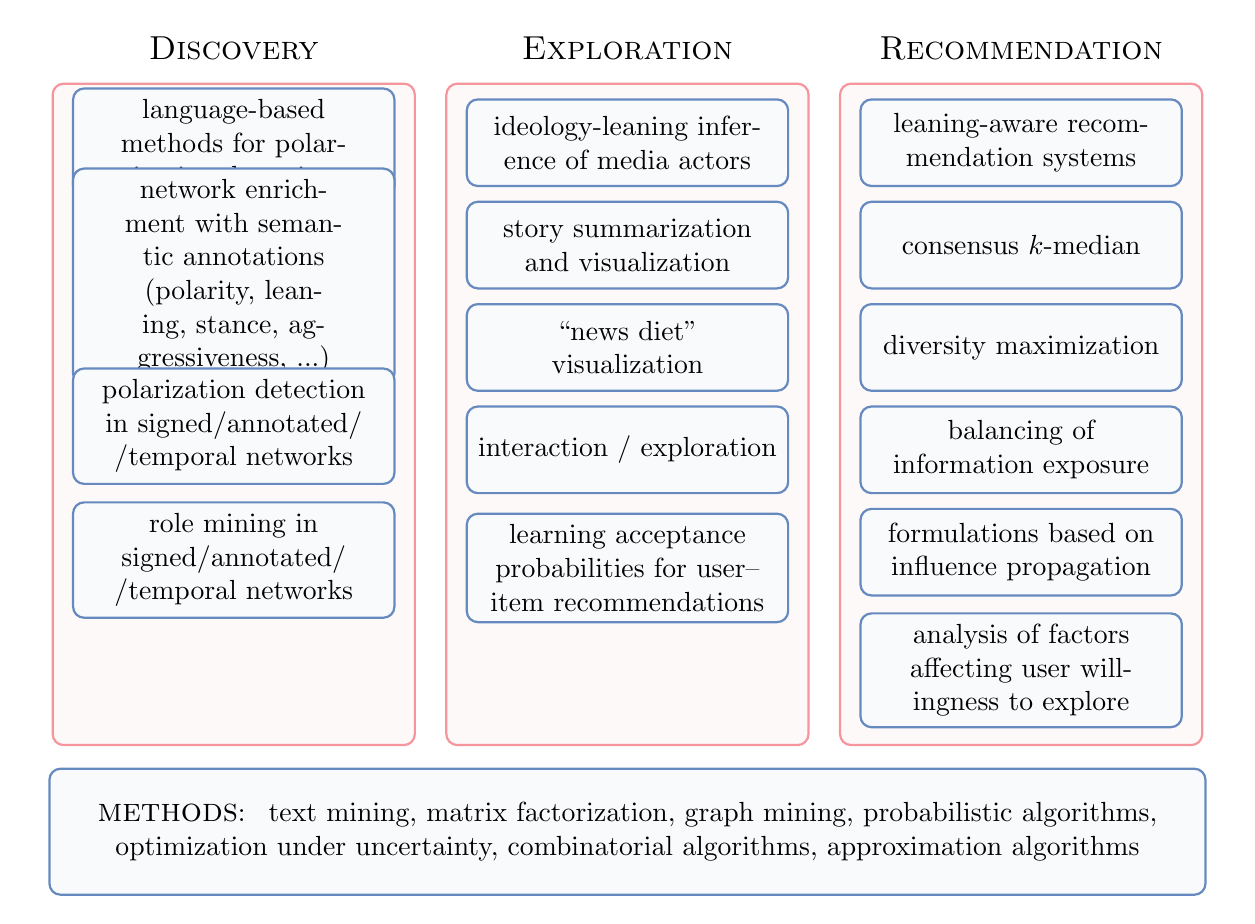
\begin{tikzpicture}
  [auto,
  frame/.style ={draw=yafcolor4!50, fill=yafcolor4!03, thick, inner sep=0em, rounded corners, text centered,
    text width=4.6cm, minimum height=8.4cm},
  block/.style ={draw=yafcolor5!70, fill=yafcolor5!03, thick, inner sep=0.4em, rounded corners, text centered,
    text width=3.8cm, minimum height=1.1cm}, 
  plaintext/.style = {text width=1.8cm, text centered},
  widetext/.style = {text width=5cm, text centered},    
  ]

\tikzstyle{simpleline} = [color=yafcolor4!70, thick, dashed]

\node[frame] (f1) at (5,2.55) {};
\node[widetext] (rh1) at (5,7.2) {\discover};

\node[block] (b11) at (5,6)   { language-based methods for polarization detection } ;
\node[block] (b12) at (5,4.3) { network enrichment with semantic annotations\\(polarity, leaning, stance, aggressiveness, ...) } ;
\node[block] (b13) at (5,2.4) { polarization detection in signed/annotated/ /temporal networks } ;
\node[block] (b14) at (5,0.7) { role mining in signed/annotated/ /temporal networks } ;


\node[frame] (f2) at (10,2.55) {};
\node[widetext] (rh2) at (10,7.2) {\explore};

\node[block] (b21) at (10,6)   { ideology-leaning inference of media actors } ;
\node[block] (b21) at (10,4.7) { story summarization and visualization } ;
\node[block] (b23) at (10,3.4) { ``news diet'' visualization } ;
\node[block] (b24) at (10,2.1) { interaction / exploration } ;
\node[block] (b25) at (10,0.6) { learning acceptance probabilities for user--item recommendations  } ;


\node[frame] (f3) at (15,2.55) {};
\node[widetext] (rh3) at (15,7.2) {\recommend};

\node[block] (b31) at (15,6)   { leaning-aware recommendation systems } ;
\node[block] (b31) at (15,4.7) { consensus $k$-median } ;
\node[block] (b33) at (15,3.4) { diversity maximization } ;
\node[block] (b34) at (15,2.1) { balancing of\\information exposure } ;
\node[block] (b35) at (15,0.8) { formulations based on influence propagation } ;
\node[block] (b35) at (15,-0.7) { analysis of factors affecting user willingness to explore  } ;


\node[block, text width=14.4cm, minimum height=1.6cm] (b35) at (10,-2.75) 
	{ \methods :~ text mining, matrix factorization, graph mining, 
	probabilistic algorithms, optimization under uncertainty, 
	combinatorial algorithms, approximation algorithms } ;

\end{tikzpicture}
}
\caption{\label{figure:structure}
The structure of {\acronym}, depicting the research thrusts of the project, 
the problem formulations we will consider, and the methods we will employ.}
\end{center}
\vspace{-4mm}
\end{figure}

The project is structured in three {\em research thrusts}:
\discover, \explore, and \recommend.
Each thrust specifies a research domain within the project
and a set of concrete problems with common motivation and common vision.
While to a large extent the problems within each thrust can be studied independently, 
there are also strong connections and feedback from one thrust will be used to obtain 
higher-quality results in the other.
The structure of the project is shown in Figure~\ref{figure:structure}.
In addition to the problems we will study within each thrust, 
we also show the computational methods that we will employ. 
% use to obtain solutions for these problems. 

\smallskip
With respect to methods, 
emphasis will be given to combinatorial algorithms,
building on the previous work of the PI 
on developing combinatorial methods for data-mining problems.
In particular, we will consider techniques such as 
combinatorial optimization, 
optimization of submodular functions, 
local-search methods, 
greedy algorithms, 
dynamic pro\-gram\-ming, 
linear-pro\-gram\-ming and semi\-def\-ini\-te-pro\-gram\-ming relaxations, 
primal-dual methods, convex optimization, etc. 
In addition, to deal with the stochastic nature of the data 
we will develop probabilistic models and algorithms that handle uncertainty.
We will also focus on designing scalable methods, 
by applying techniques based on sampling and sketching~\cite{cormode2011synopses}. 
The project also requires expertise on text analysis, 
natural-language processing, visualization, and user studies. 
These needs will be covered by hiring postdoctoral researchers with relevant expertise.

\smallskip
Next we overview the three research thrusts of \acronym.

\subsubsection*{Research thrust 1: \discover}

\noindent
\hspace{-3mm}\colorbox{verylightmagenta}{
\begin{minipage}{\textwidth}
In this research thrust we will develop novel computational methods 
to discover patterns and structure related to 
bias, polarization, conflict, and information silos in online media.
We will focus on mining se\-man\-ti\-cal\-ly-annotated graphs
with information extracted by text analysis, 
mining dynamic and temporal networks, 
and understanding the roles of individuals 
during the information-dissemination process. 
\end{minipage}}

\medskip
This thrust builds strongly on our preliminary work.
In particular, we have considered the problem 
of identifying controversial discussions on social media~\cite{garimella2018quantifying}.
Our methods are designed to be applicable to topics in any domain 
(e.g., political, economical, or cultural), and in a general setting.
We have also addressed the question of devising a measure of controversy,
which is applicable to any online discussion.
More recently we devised a new study aimed to 
understand the phenomenon of echo chambers in social media, 
and to characterize distinct user types and their role in their local community~\cite{garimella2018political}.

\smallskip
In this project we will extend significantly our problem representations
so as to obtain a deeper analysis and develop much more advanced knowledge-discovery methods.
In particular, our existing work relies on analyzing plain graphs
with no additional information regarding text or time. 
In \acronym\ we will incorporate text information into the mining process.
We will develop methods to extract semantic annotations from the textual data, 
such as
($i$) agreement between users; 
($ii$) political leaning of users or content items; 
($iii$) stance with respect to topics; 
and so on.
We will use this information to enrich our graph models,
provide novel formulations for mining semantically-annotated graphs, 
and then design efficient algorithms.

\smallskip
As an example, we will consider discussion graphs
where edges are annotated with agreement (`$+$') or disagreement (`$-$'), 
and thus, represented as {\em signed graphs}.
In this setting we will consider the problems of discovering alliances 
(dense subgraphs with many `$+$' and few `$-$' edges) 
or conflicting communities
(sets of vertices with many `$+$' and few `$-$' within sets and many `$-$' and few `$+$' across sets). 
These are novel problems related to dense-subgraph discovery~\cite{rozenshtein2014event,sozio2010community-search,tatti2015density,tsourakakis2013denser}
and correlation clustering~\cite{bansal2004correlation,gionis2007clustering}.

\smallskip
We will also leverage the temporal dimension of the data
and study formulations that allow to model and discover 
bias, polarization, and conflict in the setting of temporal networks.
This thread will make strong connections with our previous work on 
temporal networks~\cite{rozenshtein2016temporal, rozenshtein2016reconstructing, rozenshtein2017finding}
Finally we will consider problem representations  
related to motif discovery~\cite{aslay2018mining,coletto2017motif} and role mining~\cite{arockiasamy2016combinatorial} 
in the context of \acronym.


\subsubsection*{Research thrust 2: \explore}

\noindent
\hspace{-3mm}\colorbox{verylightmagenta}{
\begin{minipage}{\textwidth}
In this research thrust we will develop methods to help users 
understand better the global information landscape with respect to topics of their interest, 
visualize stories with annotations about different viewpoints, and 
increase their awareness about existing bias in the content they consume.
\end{minipage}}

\medskip
The underlying idea here is to allow users to visualize their content consumption
so that they become aware of possible biases in their ``news diet.'' 
At the same time we want to provide them the capability to visualize 
a more wide spectrum of information regarding a topic,
and support them explore alternative viewpoints.
Our preliminary work in this thrust
includes a novel method for inferring political-leaning scores
for user accounts and content sources in social media, 
in a completely unsupervised manner~\cite{lahoti2018joint}.
Those scores can be used in a number of different applications
involving information-retrieval tasks or content visualization and exploration.

\smallskip
In \acronym\ we will push this direction significantly beyond the state of the art. 
We will develop methods that produce comprehensive and understandable summaries 
of topics of interest discussed in online media. 
Our story summaries will contain information regarding the timeline of relevant events, 
important actors, entities, or concepts involved in the story, 
key persons participating in the discussion, and 
pointers to informative content. 
The summaries we will produce will allow users to understand
($i$) how polarized is a given topic;
($ii$) what is the spectrum of opinions about the topic;
($iii$) who are the most authoritative actors supporting a given opinion; 
($iv$) what is best available content for that opinion;
($v$) what is the bias/position of media outlets regarding a topic; 
and so on. 
In addition, our framework will allow users to visualize their own position in the opinion space
based on the content they have been exposed, 
their interaction with other users, and the content they have shared.

\smallskip
Finally, leveraging our framework for exploration and interaction 
% with content presented to the users, 
we will develop methods to learn the probability 
that a certain user is interested in exploring a given information item.
These probabilities will be used to optimize relevance of recommendations
in the third~thrust.


\subsubsection*{Research thrust 3: \recommend}

\noindent
\hspace{-3mm}\colorbox{verylightmagenta}{
\begin{minipage}{\textwidth}
In this research thrust we will 
develop recommendation algorithms that aim to increase the overall diversity in the network and 
balance information exposure of conflicting views. 
We will also investigate the effect of different features 
to the willingness of the users to explore viewpoints that conflict their opinion.
\end{minipage}}

\medskip
Again, this thrust is strongly based on our preliminary results.
In one of our most recent works we considered the problem of 
selecting a set of representative content items
(such as, news articles with varying opinions on a given topic)
to summarize a larger set of items~\cite{consensus-k-median}. 
This is a standard clustering problem, 
but in addition we require to select representative items
that are close to each other,
and thus, they are not polarized.
For the resulting problem we are able to provide scalable
algorithms with approximation guarantees
and show practical relevance in the application scenario
of selecting non-polarized representatives.

\smallskip
Additionally, we have studied the setting where
we ask to make relevant recommendations to users, 
which however have positive externalities to the whole network.
In particular,
we have addressed the problems
of balancing information exposure of different viewpoints in the network~\cite{garimella2017balancing},
and maximizing network diversity, 
where diversity is measured in different ways~\cite{diversity-cascade,diversity-static}.

\smallskip
In \acronym\ we will advance the state of the art in many directions.
First, we will enrich our networks with semantic annotations 
and will address recommendation problems in more realistic models. 
We will relax our assumptions and we will consider settings with multiple viewpoints, 
continuous polarity scores, 
and more complex information-propagation models.
We will study novel recommendation problems, 
and will seek to resolve open problems in our current problem formulations.

\subsection*{Section c. Timeliness, feasibility, and contingency planning}

As it is becoming apparent that social-media platforms have many adverse consequences,
including bias, polarization, conflict, and creation of information silos, 
and as stakeholders are raising their voices to get those problems fixed, 
achieving viable solutions will require cooperation among companies, policy makers, 
and scientists in multiple disciplines, including academic computer scientists. 
In this respect, the project is extremely timely.

\smallskip 
The PI is in a unique position to accomplish the goals of the project. 
His profile brings together 
the\-o\-ret\-i\-cal work on algorithms design,
with development of practical data-mining methods, 
and strong emphasis on applications.
The practical aspect is further enhanced by a six-year experience in industrial research 
(Yahoo!\ Research)
and a network of collaborators in big social-media companies.
The PI is leading a research team of seven people, 
has been successful in international recruitment, 
and his doctoral students have acquired internship positions in companies
like Google, Facebook, Amazon, LinkedIn, etc.
Recent graduates are currently working in Google, EPFL, 
and University of Helsinki (assistant professor).

\smallskip 
The PI and his research team have pioneered a line of work on the project theme
and have obtained several preliminary results~\cite{diversity-cascade,garimella2017reducing,garimella2017balancing,garimella2018quantifying,lahoti2018joint,diversity-static}.
The objective of this project is to advance the state of the art in this important topic
on multiple fronts. 
In particular, we aim to work on more realistic models, 
achieve stronger algorithmic results, 
and resolve open problems. 
We also aim to enlarge and strengthen the team with researchers of complementary skills, 
and establish collaborations with industrial partners and scientists in other disciplines.
Without the support of this project it will not be possible to accomplish these ambitious goals.

\smallskip 
The research team has strong experience in collecting data from platforms like twitter and reddit, 
and much of our recent work has built on extensive data gathering.
In addition, we will seek to establish collaborations with international online-media companies
so that we can test our methods on real-world scenarios. 
We will also will seek collaboration with local media companies in Helsinki, 
such as
Yle (Finland's national public broadcasting company)
and Sanoma (a leading media group in the Nordic countries).


\mpara{Risks.}
\acronym\ sets ambitious goals and has high potential, 
but at the same time it contains significant risks.
One of our risks is the possibility 
that a majority of people prefer to receive biased content
and are not interested to explore conflicting viewpoints.
This would be an in\-ter\-est\-ing finding for the project.
In this case, our knowledge-discovery methods will still be useful, 
but many of the the tools we will build they will be of interest to a smaller population.
A second risk is that we will not be successful in devising 
algorithms with quality guarantees for the most challenging problems. 
In this case, we will make simplifying assumptions and 
focus on devising heuristic methods. 
A third risk is that we will not be able to establish high-profile industrial collaborations. 
In this case, we will perform our analysis on datasets we will collect, 
or public datasets, and will evaluate our algorithms using user studies. 

\newpage
{\footnotesize
\setlength{\bibsep}{0pt}
\bibliographystyle{abbrv}
\bibliography{references}
}


\end{document}




